% Slide 41: left-side diagram only (step 1)
\begin{frame}{Method}
\begin{flushleft}
\hspace*{0.04\textwidth}%
\begin{tikzpicture}
  \node[inner sep=0] (diag) {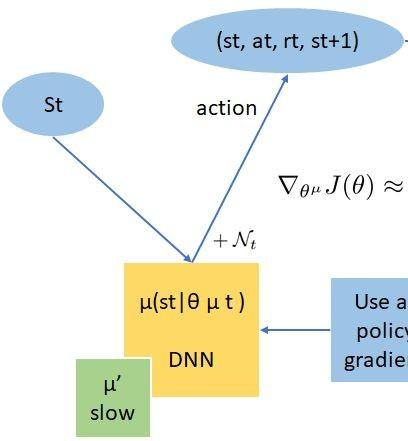
\includegraphics[width=0.42\textwidth]{images/ddpg/figures/method-flow-step1.jpg}};
  \begin{scope}[shift={(diag.south west)}, x={($(diag.south east)-(diag.south west)$)}, y={($(diag.north west)-(diag.south west)$)}]
    % Red dashed bounding rectangle around the trainable left diagram
    \draw[red, line width=1pt, dashed] (-0.02, -0.04) rectangle (0.78, 1.05);
  \end{scope}
\end{tikzpicture}
\end{flushleft}
\begin{flushright}\tiny Credit: Professor Animesh Garg\end{flushright}
\end{frame}

% Slide 42: step3 image with right Q-stuff hidden behind white overlay
\begin{frame}{Method}
\centering
\begin{tikzpicture}
  \node[inner sep=0] (diag) {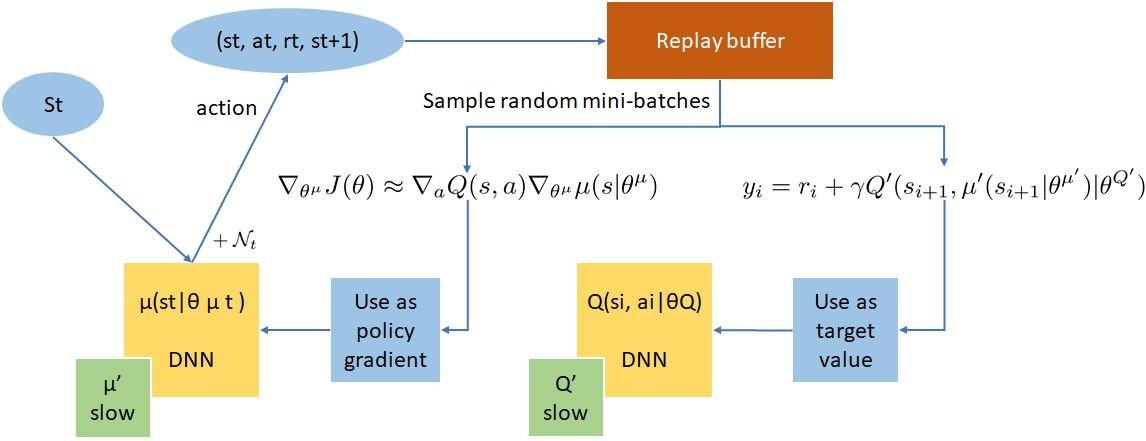
\includegraphics[width=0.95\textwidth]{images/ddpg/figures/method-flow-step3.jpg}};
  \begin{scope}[shift={(diag.south west)}, x={($(diag.south east)-(diag.south west)$)}, y={($(diag.north west)-(diag.south west)$)}]
    % Hide everything to the right of the left diagram and below the replay buffer line
    \fill[white] (0.45, 0.0) rectangle (1.05, 0.70);
    % Hide the policy-gradient formula in the middle
    \fill[white] (0.20, 0.45) rectangle (0.60, 0.72);
    % Hide the "Use as policy gradient" label between mu DNN and formula
    \fill[white] (0.22, 0.05) rectangle (0.55, 0.45);
    % Red dashed rectangle around what's visible (left trainable + replay buffer line)
    \draw[red, line width=1pt, dashed] (-0.02, -0.04) rectangle (0.55, 1.04);
  \end{scope}
\end{tikzpicture}
\begin{flushright}\tiny Credit: Professor Animesh Garg\end{flushright}
\end{frame}

% Slide 43: full method diagram
\begin{frame}{Method}
\centering
\begin{tikzpicture}
  \node[inner sep=0] (diag) {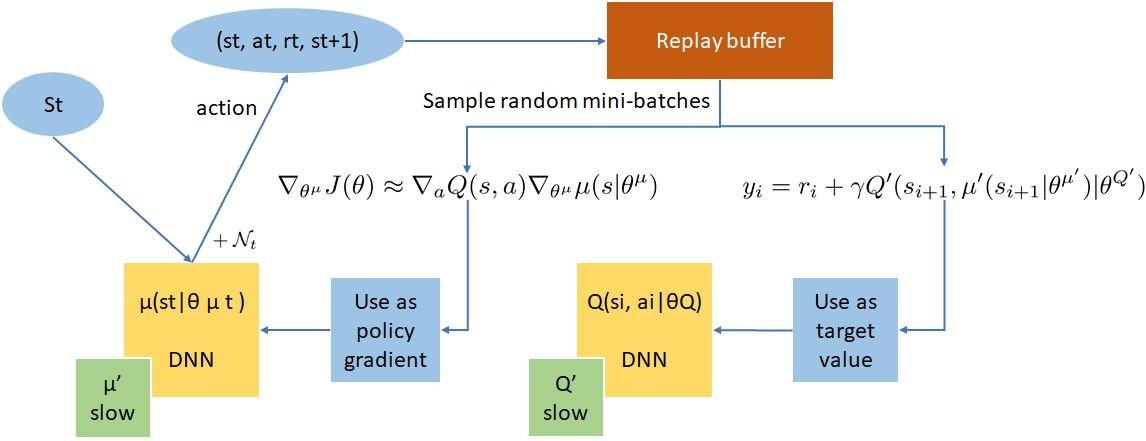
\includegraphics[width=0.95\textwidth]{images/ddpg/figures/method-flow-step3.jpg}};
  \begin{scope}[shift={(diag.south west)}, x={($(diag.south east)-(diag.south west)$)}, y={($(diag.north west)-(diag.south west)$)}]
    % Red dashed rectangle around the right-side learning loop (matches original)
    \draw[red, line width=1pt, dashed] (0.16, -0.04) rectangle (1.02, 1.04);
  \end{scope}
\end{tikzpicture}
\begin{flushright}\tiny Credit: Professor Animesh Garg\end{flushright}
\end{frame}

% Slide 44: DDPG algorithm pseudocode (no annotations)
\begin{frame}{Method}
\begin{figure}
    \centering
    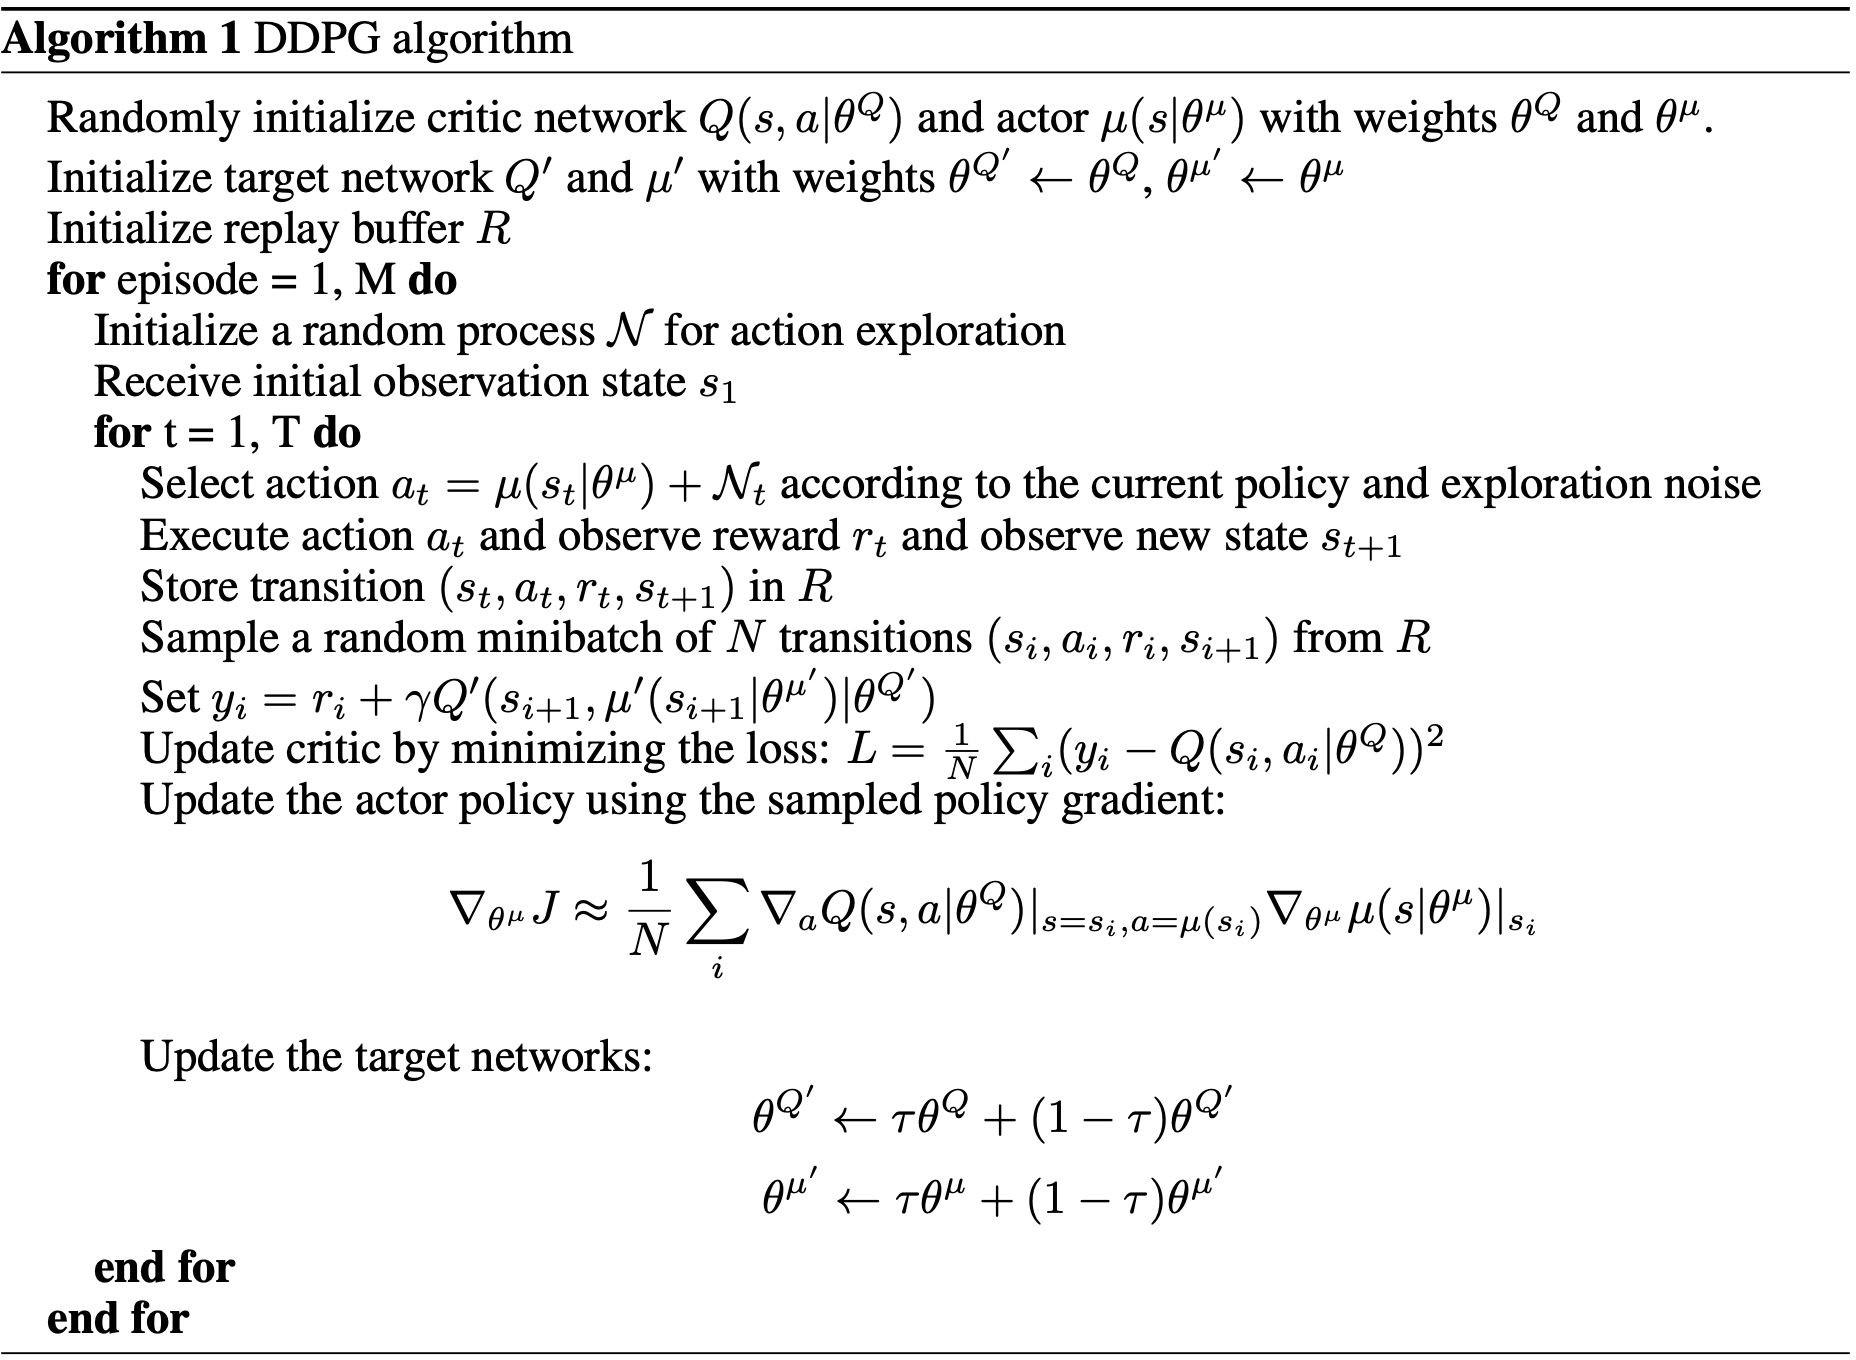
\includegraphics[width=0.80\textwidth,height=0.85\textheight,keepaspectratio]{images/ddpg/figures/ddpg-algorithm.jpg}
\end{figure}
\end{frame}

% Slide 45: replay buffer + soft target network update boxes
\begin{frame}{Method}
\begin{columns}[c]
\begin{column}{0.18\textwidth}
\centering
\textbf{Replay buffer}\\[3em]
\textbf{``Soft'' target network update}
\end{column}
\begin{column}{0.82\textwidth}
\centering
\begin{tikzpicture}
\node[inner sep=0] (algo) {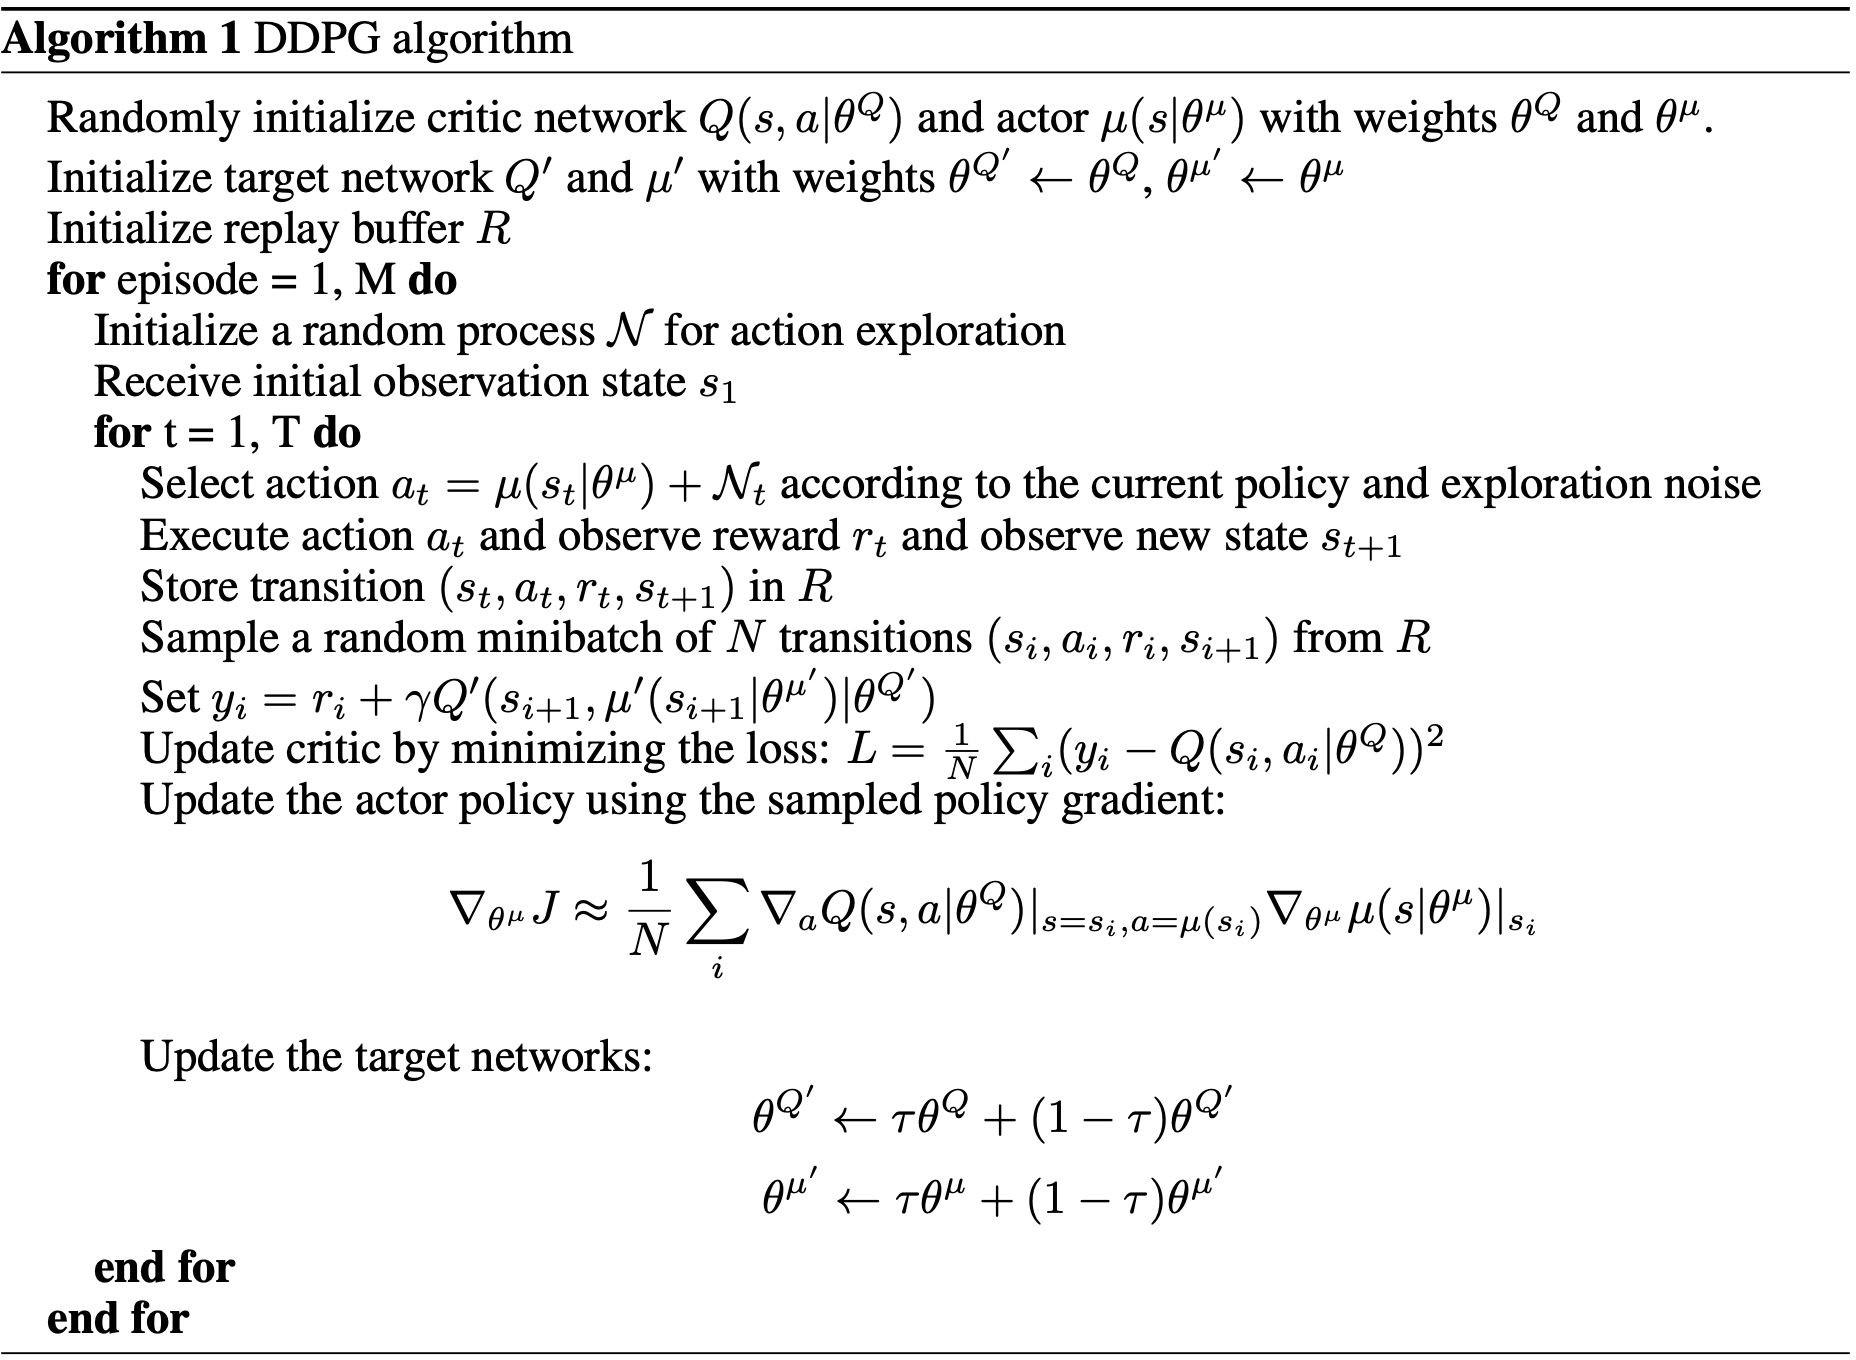
\includegraphics[width=\linewidth,height=0.85\textheight,keepaspectratio]{images/ddpg/figures/ddpg-algorithm.jpg}};
\begin{scope}[shift={(algo.south west)}, x={($(algo.south east)-(algo.south west)$)}, y={($(algo.north west)-(algo.south west)$)}]
  \draw[red,line width=0.7pt] (0.03, 0.80) rectangle (0.30, 0.85);
  \draw[red,line width=0.7pt] (0.18, 0.05) rectangle (0.78, 0.25);
\end{scope}
\end{tikzpicture}
\end{column}
\end{columns}
\end{frame}

% Slide 46: Add noise for exploration
\begin{frame}{Method}
\begin{columns}[c]
\begin{column}{0.18\textwidth}
\centering
\textbf{Add noise for exploration}
\end{column}
\begin{column}{0.82\textwidth}
\centering
\begin{tikzpicture}
\node[inner sep=0] (algo) {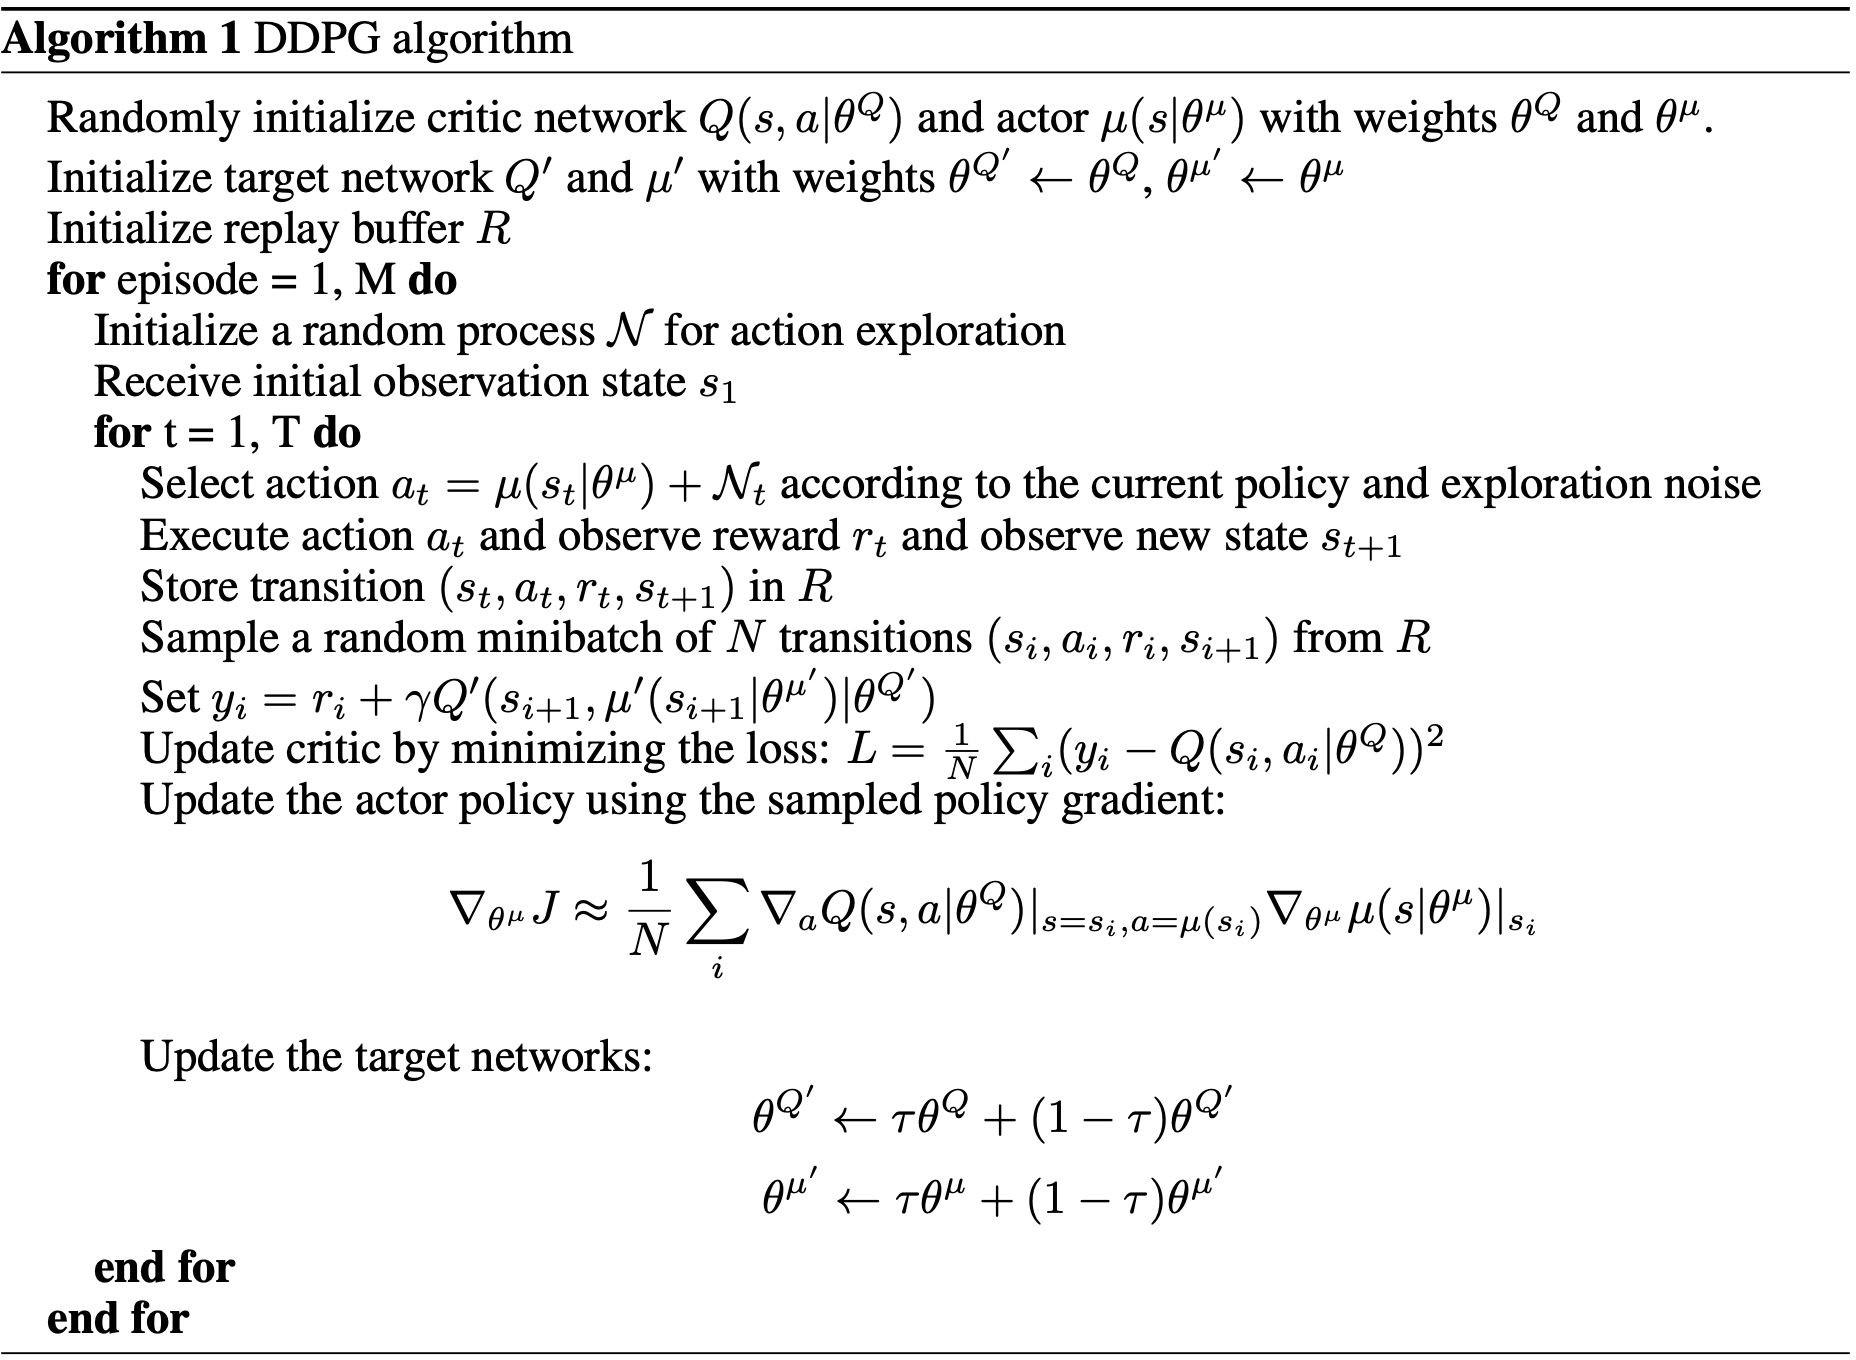
\includegraphics[width=\linewidth,height=0.85\textheight,keepaspectratio]{images/ddpg/figures/ddpg-algorithm.jpg}};
\begin{scope}[shift={(algo.south west)}, x={($(algo.south east)-(algo.south west)$)}, y={($(algo.north west)-(algo.south west)$)}]
  \draw[red,line width=0.7pt] (0.06, 0.625) rectangle (0.95, 0.675);
\end{scope}
\end{tikzpicture}
\end{column}
\end{columns}
\end{frame}

% Slide 47: Value Network Update
\begin{frame}{Method}
\begin{columns}[c]
\begin{column}{0.18\textwidth}
\centering
\textbf{Value Network Update}
\end{column}
\begin{column}{0.82\textwidth}
\centering
\begin{tikzpicture}
\node[inner sep=0] (algo) {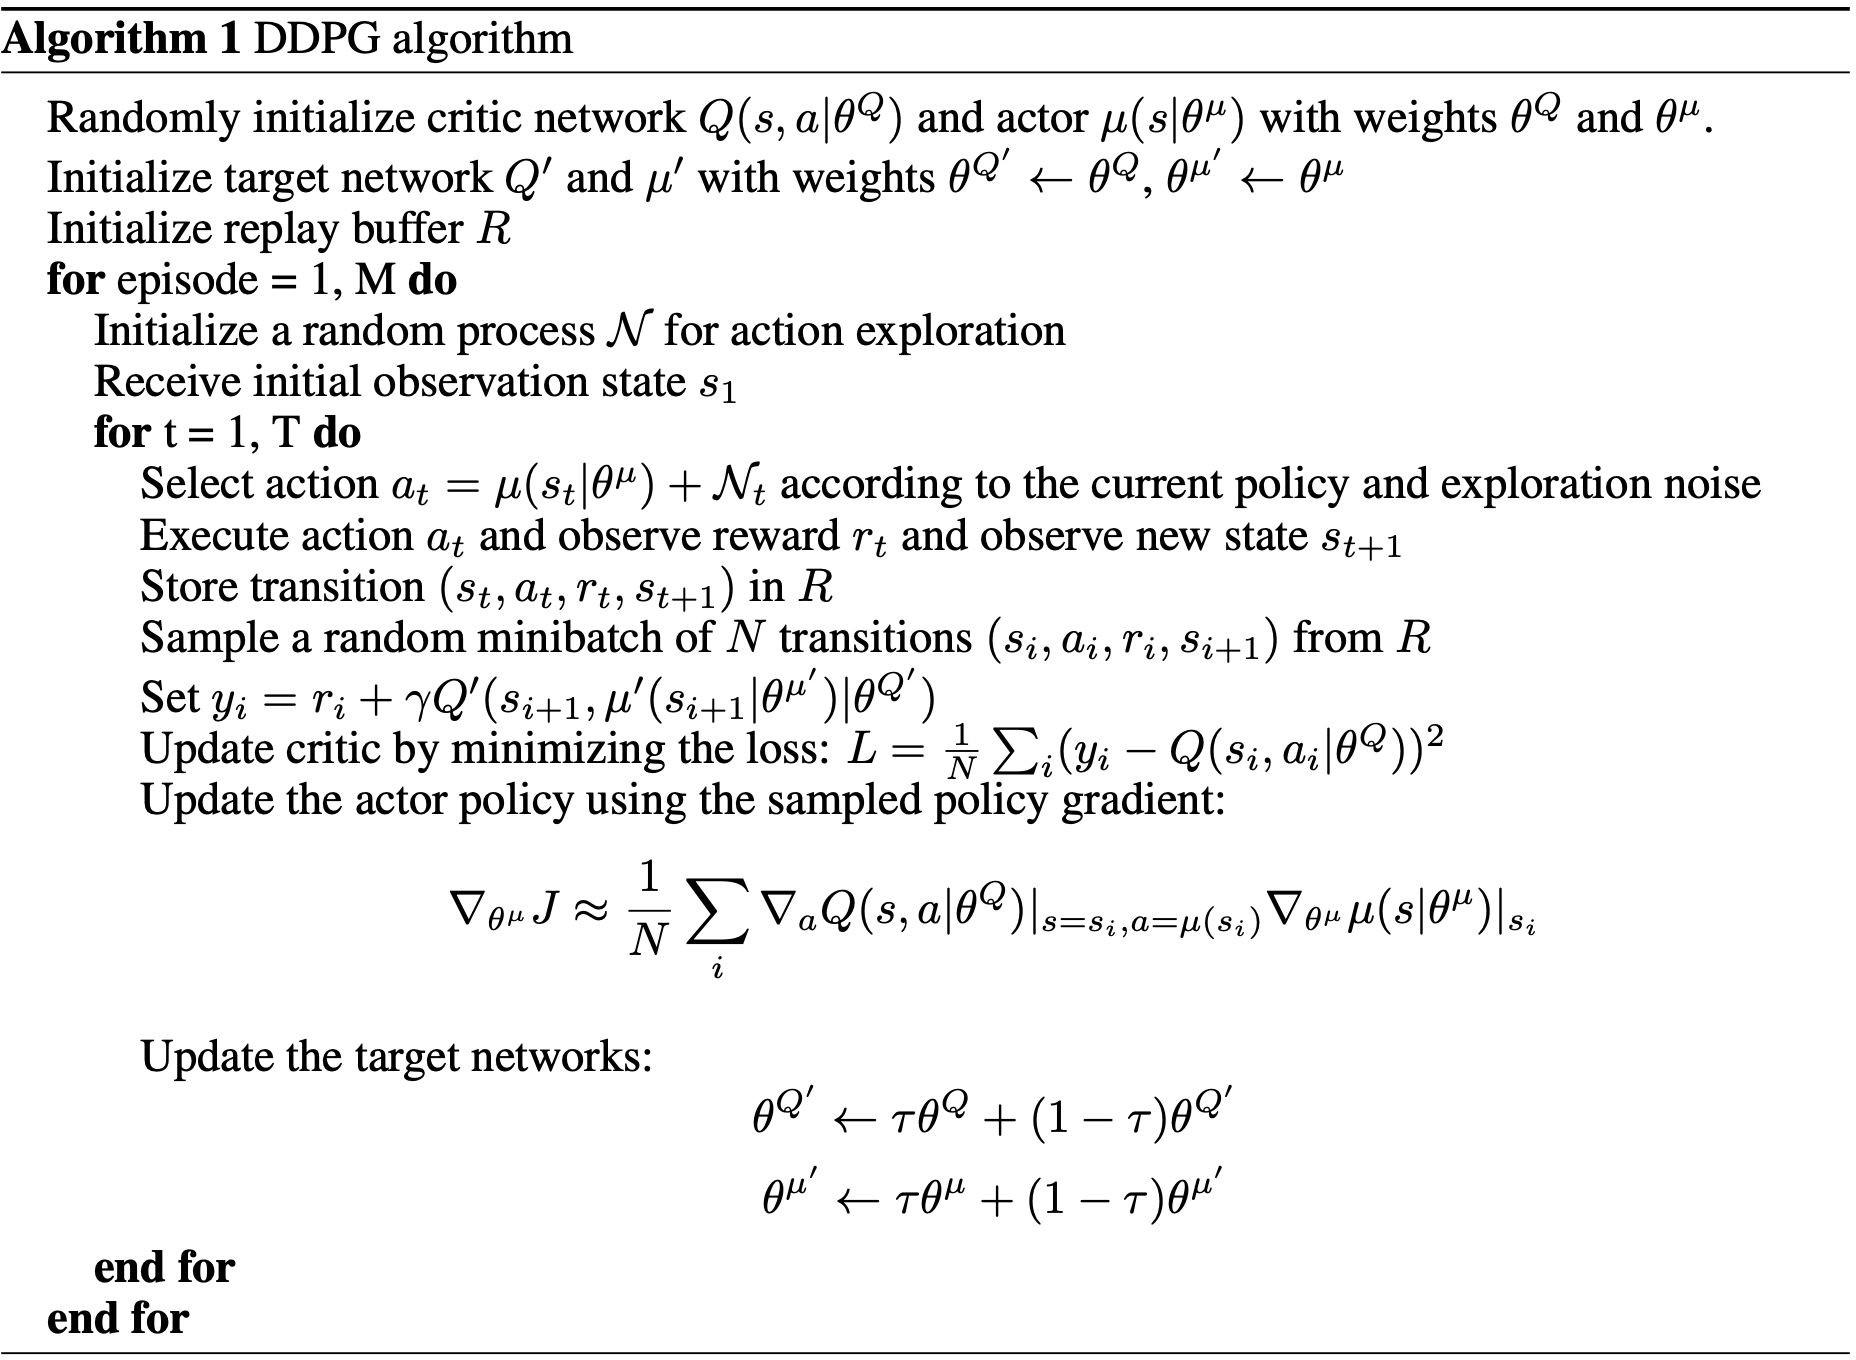
\includegraphics[width=\linewidth,height=0.85\textheight,keepaspectratio]{images/ddpg/figures/ddpg-algorithm.jpg}};
\begin{scope}[shift={(algo.south west)}, x={($(algo.south east)-(algo.south west)$)}, y={($(algo.north west)-(algo.south west)$)}]
  \draw[red,line width=0.7pt] (0.06, 0.43) rectangle (0.85, 0.54);
\end{scope}
\end{tikzpicture}
\end{column}
\end{columns}
\end{frame}

% Slide 48: Policy Network Update
\begin{frame}{Method}
\begin{columns}[c]
\begin{column}{0.18\textwidth}
\centering
\textbf{Policy Network Update}
\end{column}
\begin{column}{0.82\textwidth}
\centering
\begin{tikzpicture}
\node[inner sep=0] (algo) {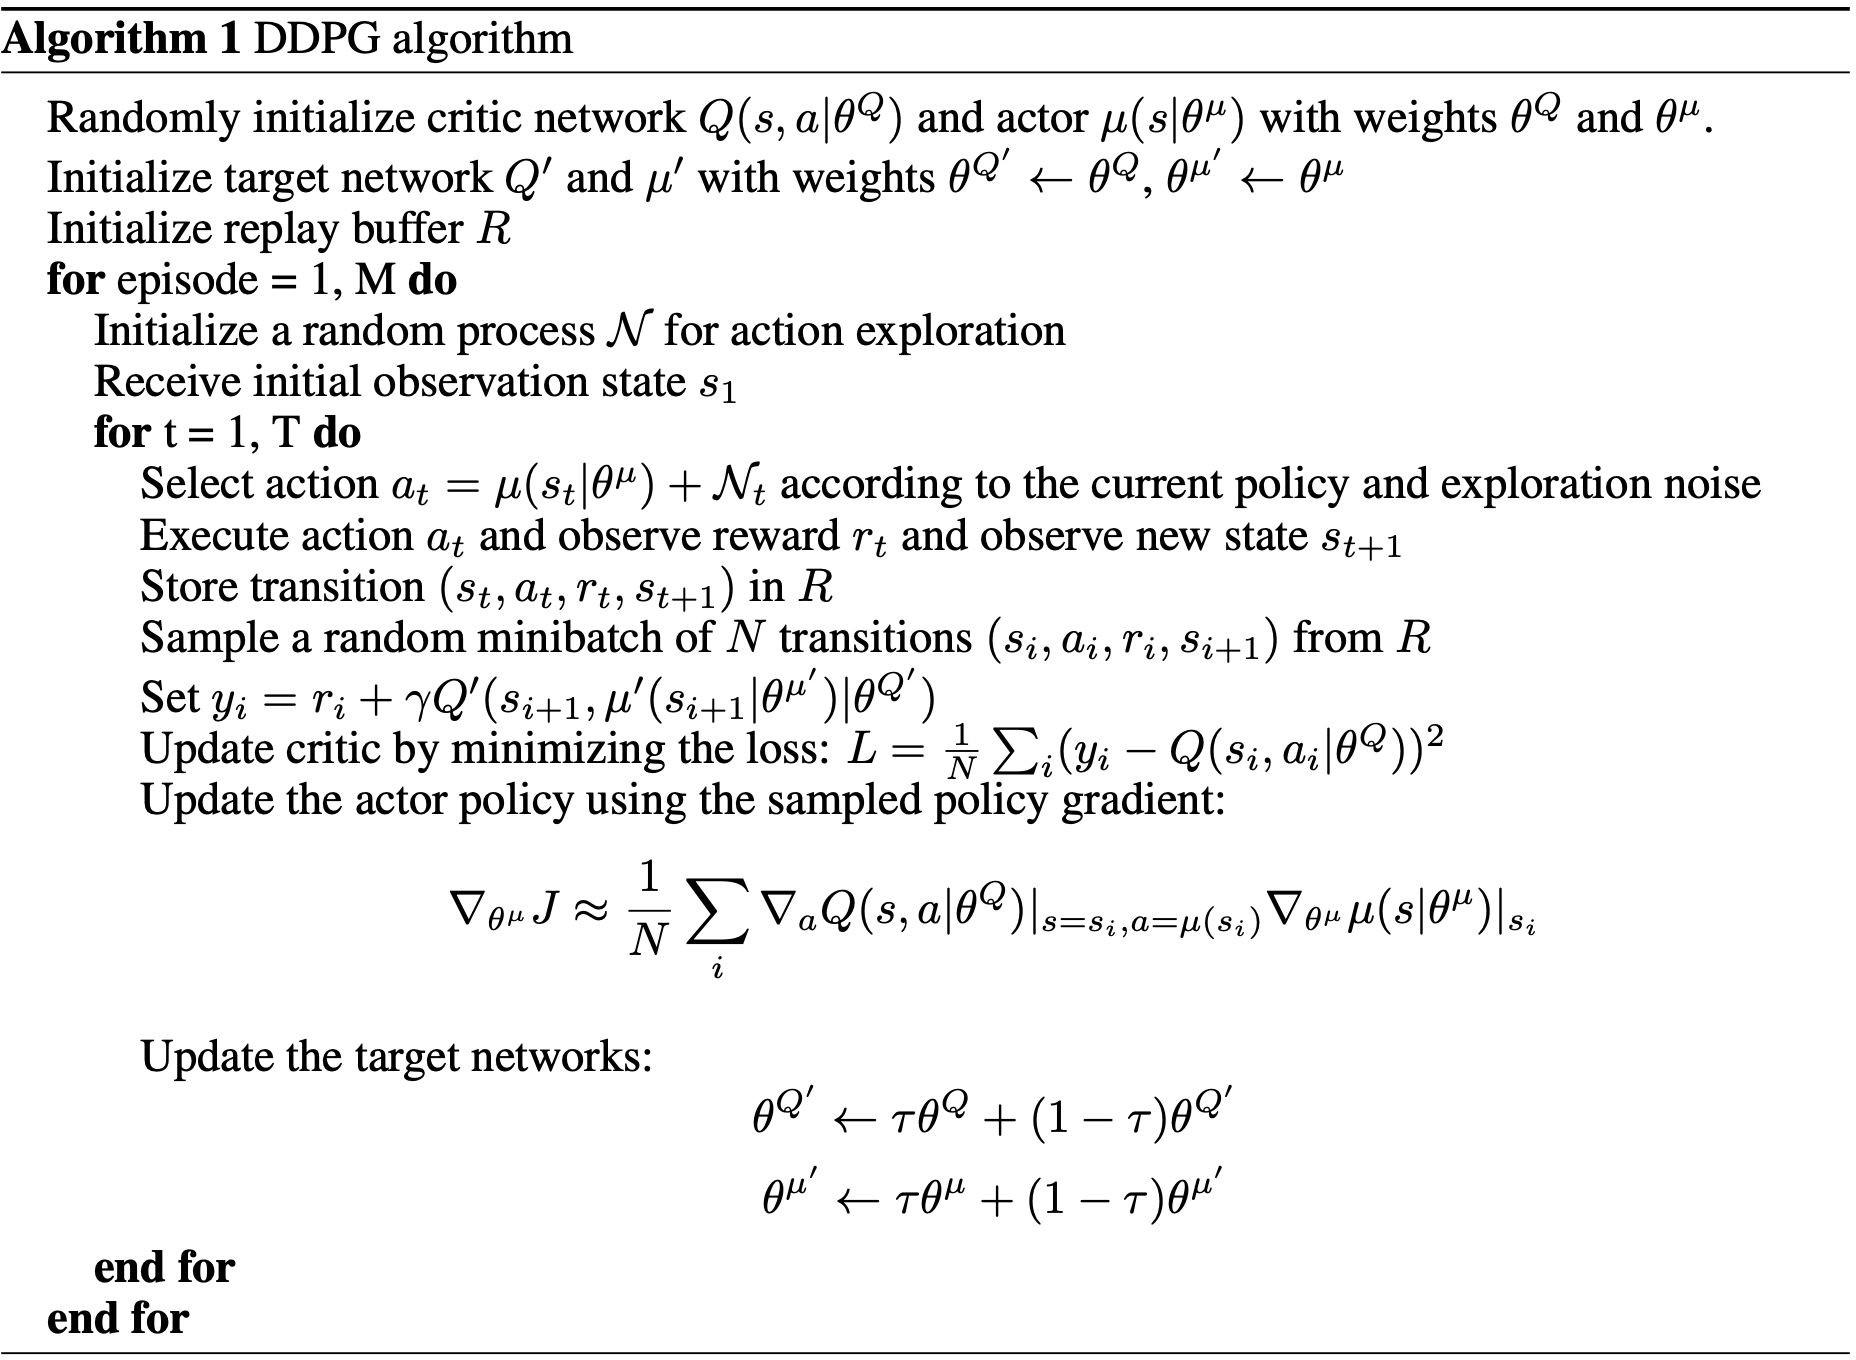
\includegraphics[width=\linewidth,height=0.85\textheight,keepaspectratio]{images/ddpg/figures/ddpg-algorithm.jpg}};
\begin{scope}[shift={(algo.south west)}, x={($(algo.south east)-(algo.south west)$)}, y={($(algo.north west)-(algo.south west)$)}]
  \draw[red,line width=0.7pt] (0.10, 0.25) rectangle (0.78, 0.36);
\end{scope}
\end{tikzpicture}
\end{column}
\end{columns}
\end{frame}

% Slide 49: DQN algorithm pseudocode with epsilon-greedy box
\begin{frame}{Method}
\begin{tikzpicture}
\node[inner sep=0] (dqn) {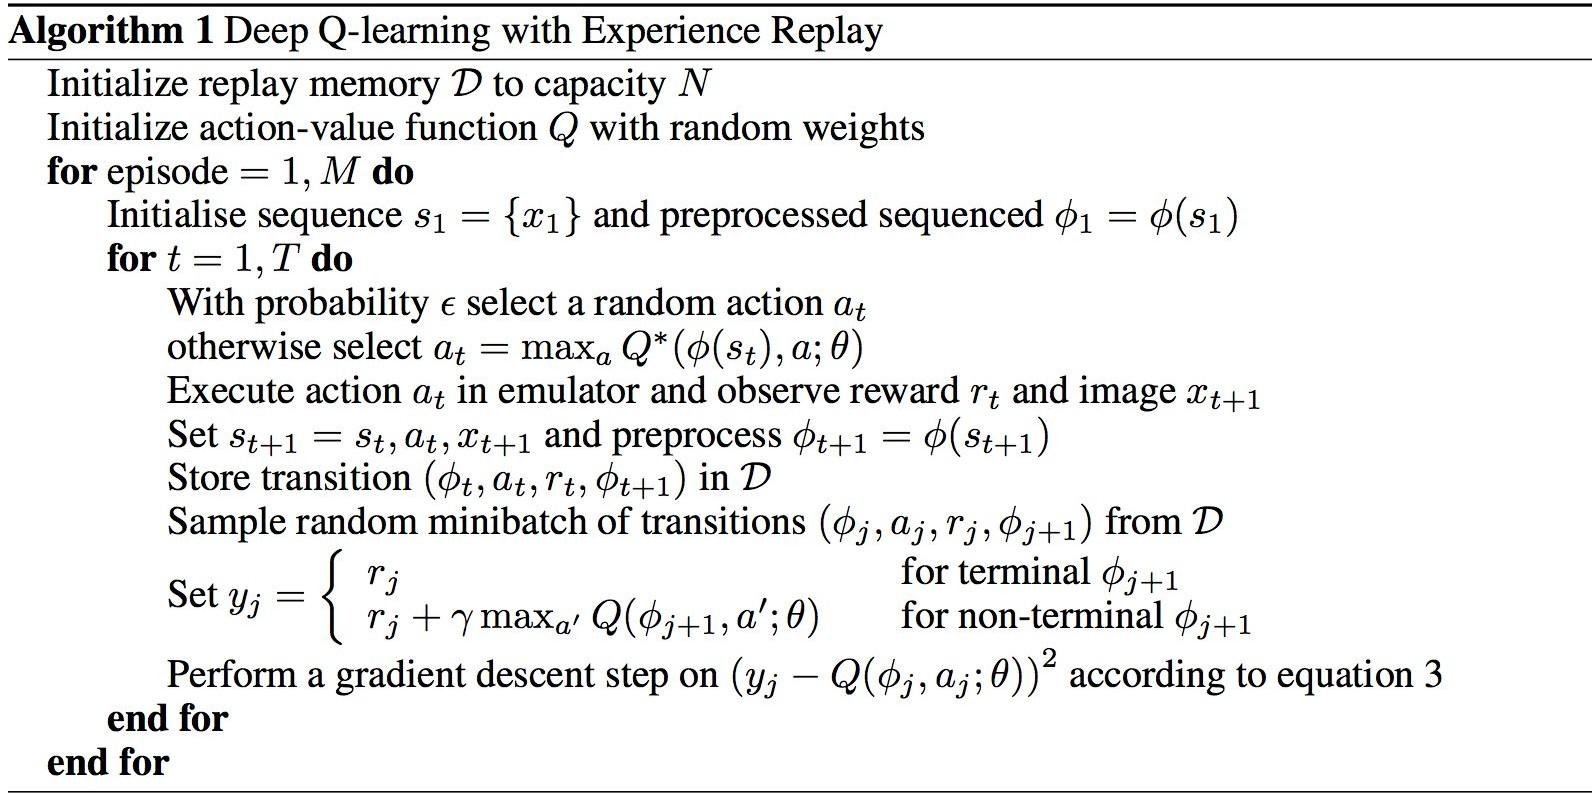
\includegraphics[width=0.85\textwidth,height=0.85\textheight,keepaspectratio]{images/ddpg/figures/dqn-algorithm.jpg}};
\begin{scope}[shift={(dqn.south west)}, x={($(dqn.south east)-(dqn.south west)$)}, y={($(dqn.north west)-(dqn.south west)$)}]
  \draw[red,line width=0.7pt] (0.08, 0.52) rectangle (0.85, 0.66);
\end{scope}
\end{tikzpicture}
\end{frame}

% Slide 50: DQN algorithm annotated with DDPG callout
\begin{frame}{Method}
\begin{tikzpicture}
\node[inner sep=0] (dqn) {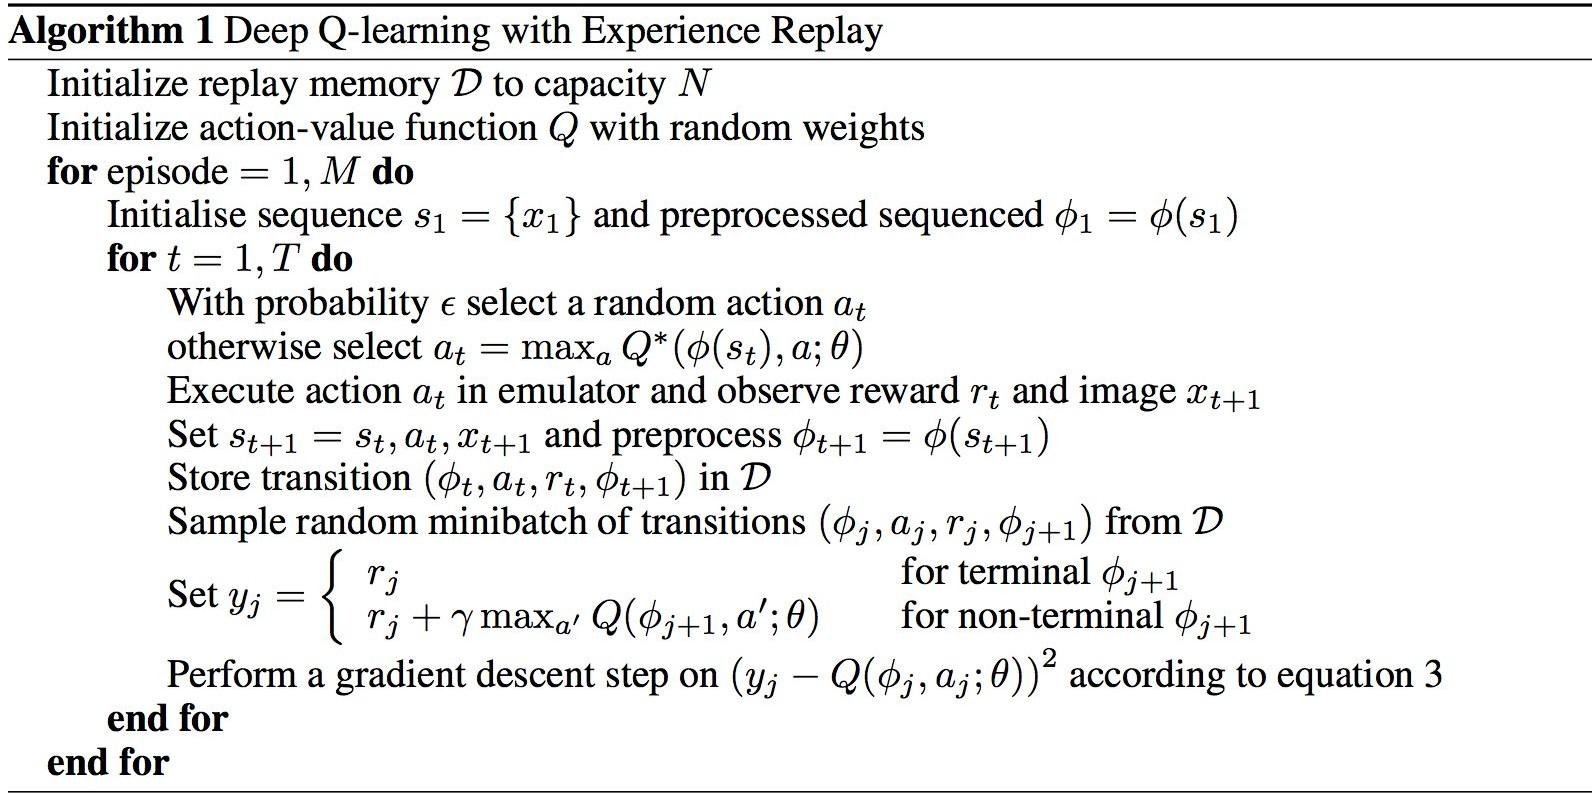
\includegraphics[width=0.85\textwidth,height=0.85\textheight,keepaspectratio]{images/ddpg/figures/dqn-algorithm.jpg}};
\begin{scope}[shift={(dqn.south west)}, x={($(dqn.south east)-(dqn.south west)$)}, y={($(dqn.north west)-(dqn.south west)$)}]
  \draw[red,line width=0.7pt] (0.08, 0.52) rectangle (0.85, 0.66);
  \node[anchor=center,fill=white,inner sep=3pt,font=\footnotesize\bfseries,text=red] at (0.46, 0.59) {DDPG: Policy Network, learned with Deterministic Policy Gradient};
\end{scope}
\end{tikzpicture}
\end{frame}
